\documentclass[14pt,final,oneside]{article}% класс документа, характеристики
%>>>>> Разметка документа
\usepackage[a4paper, mag=1000, left=3cm, right=1.5cm, top=2cm, bottom=2cm, headsep=0.7cm, footskip=1cm]{geometry} % По ГОСТу: left>=3cm, right=1cm, top=2cm, bottom=2cm,
\linespread{1} % межстройчный интервал по ГОСТу := 1.5
%<<<<< Разметка документа
\usepackage[utf8]{inputenc}
\usepackage[T2A]{fontenc}
\usepackage[english, russian]{babel}
\usepackage{amsmath, amsfonts, amssymb, amssymb, amsthm, mathtools}
\usepackage{geometry}
\usepackage{colortbl} % таблички
\usepackage{listings} % листинг
\usepackage{dcolumn} % выравнивание чисел
\usepackage[normalem]{ulem} % для подчёркиваний uline
\ULdepth = 0.16em % расстояние от линии до текста выше/ниже
\lstset{basicstyle=\ttfamily\normalsize}  
\usepackage{graphicx}
\usepackage{longtable}
\usepackage[breaklinks]{hyperref}
\usepackage{xcolor}
\usepackage{float}
\makeatletter
\def\cyrrange#1-#2{%
    \begingroup
    \count@=`#1
    \loop
    \lst@literate{\char\count@}{\char\count@}1
    \ifnum\count@<`#2
    \advance\count@\@ne
    \repeat
    \endgroup
}
\makeatother
\lstset{
    inputencoding=utf8,       % Указываем кодировку входного текста
    extendedchars=true,       % Включаем поддержку расширенных символов
    literate=%                % Настройка отображения кириллических символов
        {а}{{\selectfont а}}1
        {б}{{\selectfont б}}1
        {в}{{\selectfont в}}1
        {г}{{\selectfont г}}1
        {д}{{\selectfont д}}1
        {е}{{\selectfont е}}1
        {ё}{{\selectfont ё}}1
        {ж}{{\selectfont ж}}1
        {з}{{\selectfont з}}1
        {и}{{\selectfont и}}1
        {й}{{\selectfont й}}1
        {к}{{\selectfont к}}1
        {л}{{\selectfont л}}1
        {м}{{\selectfont м}}1
        {н}{{\selectfont н}}1
        {о}{{\selectfont о}}1
        {п}{{\selectfont п}}1
        {р}{{\selectfont р}}1
        {с}{{\selectfont с}}1
        {т}{{\selectfont т}}1
        {у}{{\selectfont у}}1
        {ф}{{\selectfont ф}}1
        {х}{{\selectfont х}}1
        {ц}{{\selectfont ц}}1
        {ч}{{\selectfont ч}}1
        {ш}{{\selectfont ш}}1
        {щ}{{\selectfont щ}}1
        {ъ}{{\selectfont ъ}}1
        {ы}{{\selectfont ы}}1
        {ь}{{\selectfont ь}}1
        {э}{{\selectfont э}}1
        {ю}{{\selectfont ю}}1
        {я}{{\selectfont я}}1
        {Б}{{\selectfont Б}}1
        {К}{{\selectfont К}}1
        {О}{{\selectfont О}}1
    language=Python,            % Язык программирования
    numbers=left,             % Нумерация строк слева
    stepnumber=1,             % Каждая строка нумеруется
    numbersep=5pt,            % Отступ от кода до номеров строк
    showspaces=false,         % Не показывать пробелы
    showstringspaces=false,   % Не показывать пробелы в строках
    tabsize=4,                % Размер табуляции
    frame=single,             % Рамка вокруг кода
    breaklines=true,          % Перенос строк
    breakatwhitespace=false,  % Переносить строки по пробелам
    basicstyle=\ttfamily,     % Шрифт текста
    keywordstyle=\color{blue},% Цвет ключевых слов
    commentstyle=\color{green},% Цвет комментариев
    stringstyle=\color{red},  % Цвет строковых литералов
}
\usepackage{minted} 

\usepackage{titlesec}
\titleformat{\section}
{\LARGE\bfseries}
{\thesection}{15pt}{} 
\usepackage{fancyhdr}
\renewcommand{\thesection}{\arabic{section}.}
\renewcommand{\thesubsection}{\arabic{section}.\arabic{subsection}.}
\usepackage{tocloft}
\renewcommand{\cftsecleader}{\cftdotfill{\cftdotsep}}
\renewcommand{\cftsecfont}{\Large\bfseries} 
\renewcommand{\cfttoctitlefont}{\LARGE\bfseries}
\newcommand{\lr}[1]{\left( {#1} \right)}
\usepackage{hyperref} % гиперссылки
\hypersetup{
    colorlinks=true,        % Включаем цветные ссылки
    linkcolor=blue!50!black, % Цвет внутренних ссылок (например, на разделы)
    urlcolor=blue!50!black,  % Цвет URL-ссылок
    citecolor=blue!50!black, % Цвет ссылок на библиографию
}
\usepackage{tikz}

% Команда для обведенного знака равенства
\newcommand{\circledequal}{%
    \mathbin{%
        \tikz[baseline=(X.base)] 
            \node[draw, circle, inner sep=0pt] (X) {$=$};%
    }%
}

\begin{document}
\thispagestyle{empty}
\begin{center}
\LARGE{Университет ИТМО} 
\vspace{20pt}

\LARGE{Факультет программной инженерии и компьютерной техники \\
Образовательная программа системное и прикладное программное обеспечение}
\vspace{160pt}

\LARGE{Лабораторная работа  \textnumero 2 \\
По дисциплине "Основы профессиональной деятельности" \\ 
Вариант 98806}
\vspace{120pt}
\end{center}

\begin{flushright}
\LARGE{Выполнил студент группы P3109 \\ 
Евграфов Артём Андреевич \\
Проверила: \\
Бострикова Дарья Константиновна}
\vspace{120pt}
\end{flushright}

\begin{center}
\Large{Санкт-Петербург 2024}
\end{center}

\newpage
\setcounter{page}{1}
\tableofcontents
\newpage
\section{Задание варианта}
\begin{figure}[H]
    \centering
    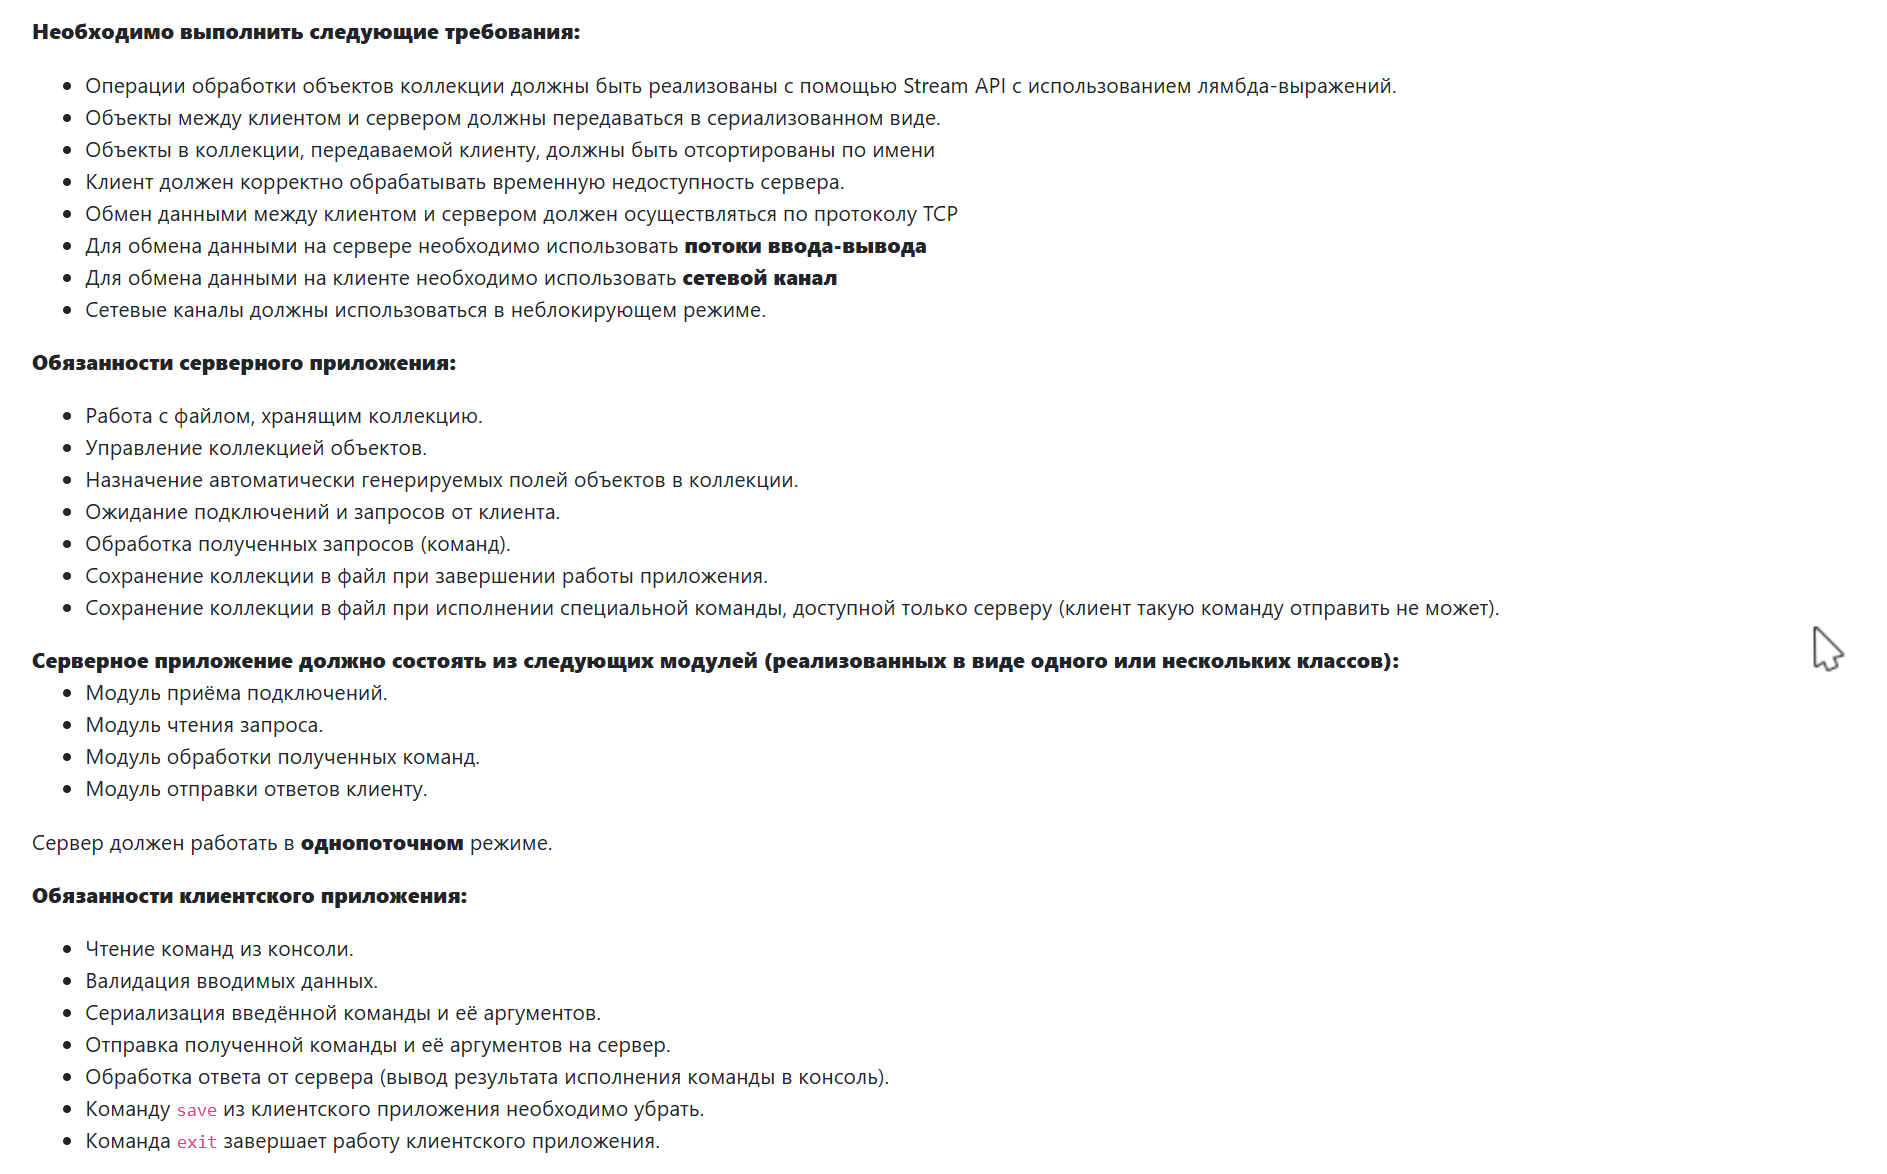
\includegraphics[width=1\linewidth]{task.png}
\end{figure}
\section{Выполнение задания}
\subsection{Текст исходной программы}
\begin{table}[H]
\centering
\begin{tabular}{|>{\centering\arraybackslash}p{1.5cm}|>{\centering\arraybackslash}p{2cm}|>{\centering\arraybackslash}p{3cm}|>{\arraybackslash}p{8cm}|}
\hline
Адрес & Код команды & Мнемоника & Комментарии \\\hline
064 & 0200 & CLA & Очистить содержимое аккумулятора \\\hline
065 & 0280 & NOT & Побитовое отрицание аккумулятора \\\hline
066 & 206F & AND 06F & Выполнить операцию логического умножения между ячейкой памяти 06F и аккумулятором. \\
& & & (06F) \& AC $\rightarrow$ AC \\\hline
067 & 206D & AND 06D & Выполнить операцию логического умножения между ячейкой памяти 06D и аккумулятором. \\
& & & (06D) \& AC $\rightarrow$ AC \\\hline
068 & E070 & ST 070 & Записать содержимое аккумулятора в ячейку 070. \\
& & & AC $\rightarrow$ (070) \\\hline
069 & A071 & LD 071 & Записать содержимое ячейки 071 в аккумулятор. \\
& & & (071) $\rightarrow$ AC \\\hline
06A & 4070 & ADD 070 & Записать сумму текущего значения аккумулятора и значения ячейки 070 в аккумулятор. \\
& & & (070) + AC $\rightarrow$ AC \\\hline
06B & E06E & ST 06E & Записать содержимое аккумулятора в ячейку 06E. \\
& & & AC $\rightarrow$ (06E) \\\hline
06C & 0100 & HLT & Остановка программы. \\\hline
\end{tabular}
\end{table}
\newpage
\subsection{Описание программы}
Назначение программы и реализуемая ею функция (формула): \\
A = ячейка памяти 06D; \\
R = ячейка памяти 06E; \\
C = ячейка памяти 06F; \\
D = ячейка памяти 070; \\
E = ячейка памяти 071; \\

\noindent AC = 0 \\
AC = 1111 1111 1111 1111 \\
AC = C \& AC \\
AC = A \& AC \\
D = AC \\
AC = E \\
AC = D + AC \\
R = AC \\

\noindent \textbf{R = (A \& С) + E}
\subsection{Вычисление ОПИ и ОДЗ}
\textbf{Область представления:} \\
R - знаковое 16-ти разрядное число \\
A, C - набор из 16 логических однобитовых значений \\
D, E - знаковое 16-ти разрядное число \\
(A \& C) - знаковое 16-ти разрядное число \\
(A \& C) + E - знаковое 16-ти разрядное число \\
Для логических операций обасть представления: \( [0; 65535] \) \\
Для арифметических операций: \( [-32768; 32767] \) \\

\noindent \textbf{Область допустимых значений:} \\
\[
\begin{cases}
E \in [-2^{14}; 2^{14} - 1] \\
(A\, \& \,C) \in [-2^{14}; 2^{14} - 1] \\
\left[
\begin{array}{l}
\begin{cases}
A_{15}\, \oplus \, A_{14} = 0 \\
C_{15}\, \oplus \, C_{14} = 0 \\
\end{cases} \\
\begin{cases}
A_{15}\, \oplus \, C_{14} = 0 \\
C_{15}\, \oplus \, A_{14} = 0 \\
\end{cases} \\
\end{array}
\right. \\

\forall i \in \{0; 1; \dots; 13\}\,\, A_{i}, C_{i} \in \{0; 1\}
\end{cases}
\]

\begin{center}
\[
\begin{cases}
E \in [2^{14}; 2^{15} - 1] \\
\left[
\begin{array}{l}
\begin{cases}
A_{15} = C_{15} = 1 \\
\forall i \in \{0; 1; \dots; 14\}\,\, A_{i}, C_{i} \in \{0; 1\} \\
\end{cases} \\
\forall i \in \{0; 1; \dots; 15\}\,\, A_{i}\, \&\, C_{i} = 0 \\
\end{array}
\right.
\end{cases}
\]
\end{center}
\[
\begin{cases}
E \in [-2^{15}; -2^{14} - 1] \\
A_{15}\, \& \, C_{15} = 0 \\
\forall i \in \{0; 1; \dots; 14\}\,\, A_{i}, C_{i} \in \{0; 1\} \\
\end{cases}
\]

\subsection{Расположение в памяти ЭВМ программы, исходных данных и результатов; адреса первой и последней команды выполняемой программы} 
Вся программа занимает 064-071 адреса \\
Исходный код программы занимает 064-06C адреса \\
Переменные занимают 06D - 071 адреса: \\
A = ячейка памяти 06D; \\
R = ячейка памяти 06E; \\
C = ячейка памяти 06F; \\
D = ячейка памяти 070; \\
E = ячейка памяти 071; \\
Промежуточный результат хранится в ячейке 070 \\
Итоговый результат хранится в ячейке 06E \\

\noindent Адрес первой команды выполняемой программы: 064 \\
Адрес последней команды выполняемой программы: 06C
\subsection{Таблица трассировки}
\begin{center}
\begin{tabular}{|c|c|c|c|c|c|c|c|c|c|c|c|}
\hline
\textbf{Адр} & \textbf{Знч} & \textbf{IP} & \textbf{CR} & \textbf{AR} & \textbf{DR} & \textbf{SP} & \textbf{BR} & \textbf{AC} & \textbf{NZVC} & \textbf{Адр} & \textbf{Знч} \\ \hline
064 & 0200 & 064 & 0000 & 000 & 0000 & 000 & 0000 & 0000 & 0100 &  &  \\ \hline
064 & 0200 & 065 & 0200 & 064 & 0200 & 000 & 0064 & 0000 & 0100 &  &  \\ \hline
065 & 0280 & 066 & 0280 & 065 & 0280 & 000 & 0065 & FFFF & 1000 &  &  \\ \hline
066 & 206F & 067 & 206F & 06F & 0280 & 000 & 0066 & 0280 & 0000 &  &  \\ \hline
067 & 206D & 068 & 206D & 06D & 4070 & 000 & 0067 & 0000 & 0100 &  &  \\ \hline
068 & E070 & 069 & E070 & 070 & 0000 & 000 & 0068 & 0000 & 0100 & 070 & 0000 \\ \hline
069 & A071 & 06A & A071 & 071 & 0280 & 000 & 0069 & 0280 & 0000 &  &  \\ \hline
06A & 4070 & 06B & 4070 & 070 & 0000 & 000 & 006A & 0280 & 0000 &  &  \\ \hline
06B & E06E & 06C & E06E & 06E & 0280 & 000 & 006B & 0280 & 0000 & 06E & 0280 \\ \hline

\end{tabular}
\end{center}
\subsection{Программа с меньшим числом команд}
\begin{table}[H]
\centering
\begin{tabular}{|>{\centering\arraybackslash}p{1.5cm}|>{\centering\arraybackslash}p{2cm}|>{\centering\arraybackslash}p{3cm}|>{\arraybackslash}p{8cm}|}
\hline
Адрес & Код команды & Мнемоника & Комментарии \\\hline
066 & A06F & LD 06F & Записать содержимое ячейки 06F в аккумулятор. \\
& & & (06F) $\rightarrow$ AC \\\hline
067 & 206D & AND 06D & Выполнить операцию логического умножения между ячейкой памяти 06D и аккумулятором. \\
& & & (06D) \& AC $\rightarrow$ AC \\\hline
068 & 4071 & ADD 071 & Записать сумму текущего значения аккумулятора и значения ячейки 071 в аккумулятор. \\
& & & (071) + AC $\rightarrow$ AC \\\hline
069 & E06E & ST 06E & Записать содержимое аккумулятора в ячейку 06E. \\
& & & AC $\rightarrow$ (06E) \\\hline
06A & 0100 & HLT & Остановка программы. \\\hline
\end{tabular}
\end{table}
\noindent \textbf{R = (A \& C) + E}
\subsection{Трассировка с новыми числами}
A = $(0\text{x}0123)_{16}$ \\
C = $(0\text{x}0666)_{16}$ \\
E = $(0\text{xFFFF})_{16}$ \\
\[
\begin{tabular}{|c|c|c|c|c|c|c|c|c|c|c|c|}
\hline
\text{Адр} & \text{Знач} & \text{IP} & \text{CR} & \text{AR} & \text{DR} & \text{SP} & \text{BR} & \text{AC} & \text{NZVC} & \text{Адр} & \text{Знач} \\ \hline
064 & 0200 & 064 & 0000 & 000 & 0000 & 000 & 0000 & 0000 & 0100 &       &       \\ \hline
064 & 0200 & 065 & 0200 & 064 & 0200 & 000 & 0064 & 0000 & 0100 &       &       \\ \hline
065 & 0280 & 066 & 0280 & 065 & 0280 & 000 & 0065 & FFFF & 1000 &       &       \\ \hline
066 & 206F & 067 & 206F & 06F & 0666 & 000 & 0066 & 0666 & 1000 &       &       \\ \hline
067 & 206D & 068 & 206D & 06D & 0123 & 000 & 0067 & 0022 & 0000 &       &       \\ \hline
068 & E070 & 069 & E070 & 070 & 0022 & 000 & 0068 & 0022 & 0000 & 070   & 0022  \\ \hline
069 & A071 & 06A & A071 & 071 & FFFF & 000 & 0069 & FFFF & 1000 &       &       \\ \hline
06A & 4070 & 06B & 4070 & 070 & 0022 & 000 & 006A & 0021 & 0001 &       &       \\ \hline
06B & E06E & 06C & E06E & 06E & 0021 & 000 & 006B & 0021 & 0001 & 06E   & 0021  \\ \hline
\end{tabular}
\]
\newpage
\noindent Проверка трассировки вручную: \\
A = $0000\,0001\,0010\,0011_{2}$ \\
C = $0000\,0110\,0110\,0110_{2}$ \\
E - $1111\,1111\,1111\,1111_{2}$ \\
A \& C = $0000\,0000\,0010\,0010$ = $0022_{16}$\\ 
(A \& C) + E = $0000\,0000\,0010\,0001$ = $0021_{16}$ \\

\noindent Результат, полученный во время выполнения программы совпадает с результатом, полученным при ручной проверке, значит ограничение значений задано верно.


\section{Вывод}
Во время выполнения данной лабораторной работы я научился работать
с некоторыми команадами ЭВМ с абсолютной адрессацией. Изучил,
как определять область представления и область допустимых значений
исходных данных и результата, составлять таблицу трассировки и переписывать исходный код программы с меньшим числом команд.

\end{document}